\chapter{Models of Anti-de Sitter (n+1)-space}
The aim of this chapter is to construct models of Lorentzian manifolds with constant sectional curvature -1 and maximal isometry group in any dimension. We are also interested in \textit{stressing} the analogies between these manifolds with the models of hyperbolic space in the Riemannian setting. We will show that hyperbolic space is \textit{naturally} embedded in Anti-de Sitter space, and we will later develop this topic in our study of earthquakes theory. After introducing the models, we are interested in studying the geometry of such manifolds: we will \textit{give} a conformal (visual) boundary to Anti-de Sitter space and we will characterize geodesics and totally geodesic subspaces. We will also introduce the notion of polarity in Anti-de Sitter space (in some sense the \textit{correct} Lorentzian correspondence between points and hyperplane, analogous to Euclidean orthogonality) and study its properties. 

\section{The quadric model}\label{section21}
We want to introduce the analogue of the hyperboloid model of hyperbolic space. Denote by $\R^{n,2}$ the real vector space $\R^{n+2}$ equipped with the quadratic form 
\[
    q_{n,2}(x)=x_1^{2}+\dots+x_n^{2}-x_{n+1}^{2}-x_{n+2}^2.   
\]
and by $\langle v,w\rangle_{n,2}$ the associated symmetric form. Finally, let $O(n,2)$ be the group of linear transformations of $\R^{n+2}$ that preserve $q_{n,2}.$
Then we define:
\[
    \H^{n,1}=\{x\in \R^{n,2}\;|\;q_{n,2}(x)=-1\}.
\]

It is immediate to check that $\H^{n,1},$ as the pre-image of a regular value of $q_{n,2}$, is a smooth connected submanifold of $\R^{n,2}$ of dimension $n+1$. The tangent space $T_x\H^{n,1}$, regarded as a subspace of $\R^{n+2}$, coincides with the orthogonal space $x^{\perp}=\{y\in \R^{n+2}\;|\;\langle x,y\rangle_{n,2}=0\}.$ A simple signature argument (along with the fact that $q_{n,2}(x)=-1$ for every $x\in\H^{n,1}$) shows that the restriction of the symmetric form $\langle .,. \rangle_{n,2}$ to $T_x\H^{n,1}$ has Lorentzian signature, hence it makes $\H^{n,1}$ a Lorentzian manifold. We remark that this model is the analogue of the hyperboloid model of hyperbolic space, in fact $\H^n$ is isometrically embedded in $\H^{n,1}$ as the submanifold defined by $x_{n+2}=0$, $x_{n+1}>0$. \\
The natural action of $O(n,2)$ on $\R^{n,2}$ preserves $\H^{n,1}$, and in facts $O(n,2)$ acts by isometries on $\H^{n,1}$. We remark that $O(n,2)$ acts transitively on $\H^{n,1}$ and that the stabilizer of a point $x$ acts transitively on the space of orthonormal bases of $T_x\H^{n,1}$. Hence $\H^{n,1}$ has maximal isometry group and Isom($\H^{n,1})\simeq O(n,2)$.\\
By Lemma \ref{maximalisometry}, $\H^{n,1}$ has constant sectional curvature. Let us now check that the sectional curvature is negative (in particular we will find $K=-1$). For this purpose, observe that the normal line in $\R^{n,2}$ to $\H^{n,1}$ at $x$ is identified with the line generated by $x$ itself. It follows that, if $v,w$ are tangent vector fields along $\H^{n,1}$, we have the orthogonal decomposition: 
\[
    (D_{v}w)(x)=(\nabla_{v}w)(x)+\langle v,w\rangle x, 
\]

where $D$ is the flat connection of $\R^{n+2}$ and $\nabla$ is the Levi-Civita connection of $\H^{n,1}$. Using the flatness of $D$ we get: 
\[
    R(u,v)w=\langle u,w\rangle v-\langle v,w\rangle u,
\]

so that 
\[
    \langle R(u,v)v,u \rangle =-(\langle u,u\rangle\langle v,v\rangle-\langle v,u\rangle^2), 
\]

and this shows that $\H^{n,1}$ has constant sectional curvature $-1$. We also remark that $\H^{n,1}$ is not simply connected, being homeomorphic to $\R^{n}\times \mathbb{S}^1$. 

\section{The ``Klein model" and its boundary}
Let us introduce a projective model, also known as the ``Klein model", for Anti-de Sitter geometry. Let us define: 
\[
    \A^{n,1}=\H^{n,1}/\{\pm \text{Id}\}.
\]

Since $\{\pm \text{Id}\}$ is the center of $O(n,2)$ (hence normal), $\A^{n,1}$ (when endowed with the Lorentzian metric induced by the quotient) has maximal isometry group by Proposition \ref{classification} and is therefore a model of constant sectional curvature $-1$. It can also be shown that the center of the isometry group of the Klein model is trivial, hence $\A^{n,1}$ is the \textit{minimal} model of AdS geometry, in the sense that any other model is a covering of $\A^{n,1}$.\\
By definition, $\A^{n,1}$ is naturally identified with a subspace of real projective space $\R \text{P}^{n+1}$, more explicitly with the subset of timelike directions of $\R^{n,2}$: 
\[
    \A^{n,1}=\{[x]\in \R \text{P}^{n+1}\;|\;q_{n,2}(x)<0\}.
\]
Like in hyperbolic geometry, the boundary of $\A^{n,1}$ in projective space is a quadric, that is the projectivization of lightlike vectors in $\R^{n,2}$. We denote this quadric by $\partial \A^{n,1}=\{[x]\in \R \text{P}^{n+1}\;|\;q_{n,2}(x)=0\}$.\\ We observe that isometries of $\A^{n,1}$ induce projective transformations which preserve $\partial \A^{n,1}$.  \\

\subsection{The conformal Lorentzian structure of the boundary}
We want to continue to develop the analogy with hyperbolic geometry and equip $\partial \A^{n,1}$ with a conformal Lorentzian structure that extends the one on $\A^{n,1}$, similar to the conformal \textit{visual boundary} in hyperbolic geometry. \\
A point $\ell \in\R\text{P}^{n+1}$ is identified with $\text{Span}(x)$ for some $x\in \R^{n,2},$ and the tangent space of real projective space has the canonical identification 

%This comes directly from Bonsante-Seppi
%where $S_{[x]}=\mathrm{Span}(x)$, while $Q_{[x]}=\R^{n+2}/S_{[x]}$.
%Indeed given $f\in\mathrm{Hom}(S_{[x]}, \R^{n+2})$ such that  $f(x)\neq -x$,  the point $[x_f]=[f(x)+x]$ does not depend on the choice of the representative $x$.
%In this way we define a natural map  $\Pi:\mathcal U_0\to\RP^{n+1}$, where $\mathcal U_0$ is a neighborhood of $0$ in $\mathrm{Hom}(S_{[x]}, \R^{n+2})$.
%The differential of $\Pi$ at $0$ is a surjetcive and its kernel is $\mathrm{Hom}(S_{[x]}, S_{[x]})$. Thus $d_0\Pi$ yields the stated identification
%$T_{[x]}\RP^{n+1}\cong\mathrm{Hom}(S_{[x]}, \R^{n+2})/\mathrm{Hom}(S_{[x]}, S_{[x]})\cong \mathrm{Hom}(S_{[x]}, Q_{[x]})$.

\[
    T_{\ell}\R\text{P}^{n+1}\simeq \text{Hom}(\ell,\R^{n+2}/\ell). 
\]

Now, if $\ell$ is timelike, we can identify $\R^{n+2}/\ell$ with $\ell^{\perp}.$ For any given local section $\sigma:\A^{n,1}\to \R^{n,2}$ of the projection $\R^{n,2}\to \A^{n,1}$, we can define a Lorentzian metric on $T\A^{n,1}$ setting:

\[
    \langle \langle f,g \rangle \rangle_{\sigma}=\langle f(\sigma[x]),g(\sigma[x])\rangle_{n,2}
\]

for $f,g\in T_{x}\A^{n,1}\simeq \text{Hom}(\ell,\ell^\perp$). If the section $\sigma$ has image in $\H^{n,1}$, then the aforementioned metric coincides with the pull-back of the metric over $\R^{n,2}$, since the differential of $\sigma $ identifies $T_{[x]}\A^{n,1}=T_x\H^{n,1}=x^\perp$. For a general section the identification does not hold, but we can recover a conformal metric via the formula: 
\begin{equation}\label{23}
    \langle \langle f,g \rangle \rangle_{\lambda\sigma}=\lambda^2\langle \langle f,g \rangle \rangle_{\sigma}
\end{equation}
for any function $\lambda$.\\
We consider now the case where $\ell=\text{Span}(x)$ is lightlike, i.e. $q_{n,2}(x)=0$. \\In this case we can not induce any natural metric on $\R^{n,2}/\ell$. However, if we let 
\[
    \mathbb{L}=\{x\in \R^{n,2}\;|\;q_{n,2}(x)=0\}
\]
be the space of lightlike vectors, then $T_x\mathbb{L}$ is precisely $\ell^{\perp}$ and contains $\ell$ itself. We have recovered a canonical identification: $T_\ell\partial\A^{n,1}\simeq\text{Hom}(\ell,\ell^{\perp }/\ell).$ The bilinear form of $\R^{n,2},$ when restricted to $\ell^{\perp},$ induces a non degenerate bilinear form (of signature $(n-1,1)$) on $\ell^\perp/\ell.$ We will denote such a restriction as $\langle v,w\rangle_{\ell^{\perp}/\ell}.$ \\
We can now define a metric on $\partial\A^{n,1}$ for any section $\sigma:\partial\A^{n,1}\to \mathbb{L}$ of the canonical projection by the formula:
\begin{equation}\label{24}
    ((f,g))_{\sigma}=\langle f(\sigma[x]),g(\sigma[x])\rangle_{\ell^{\perp}/\ell},
\end{equation}
for all $f,g\in \text{Hom}(\ell, \ell^\perp/\ell).$ This metric can be viewed as the pull-back of the metric: 
\begin{equation}\label{25}
    ((f,g))_\sigma=\langle \sigma_*(f), \sigma_{\ast} (g)\rangle_{n,2}, 
\end{equation}
since the degenerate metric on $T_x\mathbb{L}=\ell^\perp$ is, by construction, the pull-back of the metric of $\ell^{\perp}/\ell$ by the projection along the degenerate direction $\ell$.\\ 
The relation valid for the metric on $\A^{n,1}$ also holds for the metric on $\partial\A^{n,1}$, that is: 
\begin{equation}\label{26}
    ((f,g))_{\lambda\sigma}=\lambda^2((f,g))_{\sigma},
\end{equation} 
and therefore the induced conformal class over $T\partial\A^{n,1}$ is well defined and independent of the choice of $\sigma$ and equips the tangent space of the boundary with a conformal Lorentzian metric. %To conclude let us show that this conformal metric is naturally the compactification of $\A^{n,1}$. 
Let $\sigma$ be a section of the projection $\pi:\R^{n,2}\to \R\text{P}^{n+1}$ defined in a neighborhood $U$ of a point $x\in\partial\A^{n,1}$. By construction the metric $((\cdot,\cdot))_\sigma$ over $\partial\A^{n,1}\cap U$ is the limit, as $y\to x$ for $y\in\A^{n,1}\cap U,$ of the conformal metric associated to $\sigma$ defined over $\A^{n,1}\cap U$. 
% This means that if $(p_n,v_n)$ is a sequence in $T\A^{n,1}$ that converges to $(p_{\infty}, v_\infty)$ then 
\begin{observation}\label{222}
Let us make some observations about the light cone in the case of $\partial\A^{n,1}$. If $[y]\in\partial\A^{n,1}$ Equation \refeq{25} implies that the lightlike vectors in $T_{[y]}\partial\A^{n,1}$ are exactly the projection of vectors $x\in \R^{n,2}$ such that $\langle x,y\rangle_{n,2}=0$ and $q_{n,2}(x)=0$. These vectors are such that $\text{Span}(x,y)$ are totally degenerate planes in $\R^{n,2}$, equivalently they are projective lines contained in $\partial\A^{n,1}$. Therefore the light cone in $\partial\A^{n,1}$ through $[y]$ is the union of all the projective lines through $[y]$ that are contained in $\partial\A^{n,1}$.

\end{observation}


\subsection{The ``Poincaré model" for the universal cover}
We have already observed that $\H^{n,1}$, and its quotient $\A^{n,1}$, are not simply connected. We want to construct a simply connected model for AdS geometry. For this purpose we introduce the universal cover of $\H^{n,1}$ and $\A^{n,1}$.\\
Let $\H^n$ be the hyperboloid model of hyperbolic space. Then: 
\begin{equation}\label{ogcover}
    \pi(y,t)=(y_1,\dots,y_n,y_{n+1}\cos t,y_{n+2}\sin t)
\end{equation}


defines a map $\pi:\H^n\times \R\to \H^{n,1}$ which is a covering with deck transformations of the form $(y,t)\mapsto (y,t+2k\pi)$ for $k\in \Z$. We denote the covering space by $\AS^{n,1}$ and we observe that it is also the universal cover of $\A^{n,1}$, where the covering map is the composition of $\pi$ and the quotient by $\{\pm\text{Id}\}.$\\
Pulling back the Lorentzian metric over $\AS^{n,1},$ we get a simply connected Lorentzian manifold of constant curvature -1. The metric on $\AS^{n,1}$ is a warped product of the form: 
\begin{equation}\label{metric}
     \pi^*g_{\H^{n,1}}=g_{\H^n}-y_{n+1}^{2}dt^2.
\end{equation}
   

Moreover $\AS^{n,1}$ has maximal isometry group, hence we have obtained a simply connected model for AdS geometry. More precisely we have a central extension, that is a (non split) short exact sequence:
\[
    0\to \Z\to \textnormal{Isom}(\AS^{n,1})\to O(n,2)\to 1.
\]
It is sometimes convenient to express the metric \eqref{metric} using the Poincaré model of hyperbolic space. Recall that the disk model of the hyperbolic space is the unit disk $\D^n$ endowed with the conformal metric: $\frac{4}{(1-r^2)^2}\sum dx_i^2$, where $r^2=\vert x\vert^2$. In our setting the isometry between the disk and the hyperboloid model is given by: 
\begin{equation}
    (x_1,\dots, x_n)\mapsto \Big(y_1=\frac{2x_1}{1-r^2},\dots, y_n=\frac{2x_n}{1-r^2},y_{n+1}=\frac{1+r^2}{1-r^2}\Big). 
\end{equation}
The Poincaré model of AdS geometry is then the cylinder $\D^n\times \R$ endowed with the metric 
\begin{equation}\label{metricdisk}
    \frac{4}{(1-r^2)^2}(dx_1^2+\dots+dx_n^2)-\Big(\frac{1+r^2}{1-r^2}\Big)^{2}dt^2. 
\end{equation}

It follows from the definition that each slice $\{t=c\}$ is a totally geodesic copy of $\H^n$. The metric defined in \eqref{metricdisk} also shows that the vector field $\partial/\partial t$ is a timelike non-vanishing vector field on $\AS^{n,1}$, giving it the structure of a time-orientable manifold. Any choice of time orientation is preserved by the action of the deck transformations of the covering from the Poincaré to the Klein model, hence both $\H^{n,1}$ and $\A^{n,1}$ are time-orientable. \\
% \begin{observation}
%     Exception made for the central line passing through $x_1=\dots=x_n=t=0,$ vertical lines are not geodesic for the metric defined in \refeq{metricdisk}.  
% \end{observation}

% \subsection{The conformal metric of the boundary} 
% As we did with $\A^{n,1}$ we would like to give a conformal Lorentzian structure to the boundary of $\AS^{n,1}$. The construction actually works for any covering space of $\A^{n,1}.$ The covering map (we are now considering the projective model of $\H^n$)
% \[
%     \pi^{\prime} ([y_1:\dots:y_{n}:y_{n+1}],t)=[y_1:\dots:y_n:y_{n+1}\cos t:y_{n+1}\sin t]
% \]

% extends to a map $\pi^{\prime}:\H^n\cup \partial\H^n\times \R\to \A^{n,1}\cup \partial\A^{n,1}$. In order to compute the conformal structure of the boundary, we consider the map $\tau: \H^n\times \R\to\R^{n+2}$ defined by:
% \[
%     \tau([y_1:\dots:y_n:y_{n+1}],t)=(y_1/y_{n+1},\dots,y_n/y_{n+1},\cos t,\sin t)
% \]  
%  that extends to the boundary and induces a (local) section of the projection $\R^{n,2}\to \A^{n,1}$. In fact, let $\eta$ be the generator of the group of deck transformations of the covering $\pi^{\prime}:\AS^{n,1}   \to \A^{n,1}$, then $\tau$ has the equivariance $\tau\circ\eta^i=(-1)^i\tau.$   Using Equation \refeq{26}, the conformal Lorentzian metric on $\partial\AS^{n,1}$ induced by $\sigma$ by means of Equation \refeq{24} is the pull-back of a Lorentzian metric compatible with the natural conformal structure of the boundary $\partial\A^{2,1}$. Using the metric introduced in equation \refeq{metricdisk}, the formula \refeq{23} and by observing that $\tau$ differs by the hyperboloid section by the factor $y_{n+1}=\frac{1+r^2}{1-r^2},$ we obtain the expression 

%  \begin{equation}
%     \frac{4}{(1+r^2)^2}(dx_1^{2}+\dots+dx_n^2)-dt^2.
%  \end{equation}

%  This metric extends to $\overline{\D}\times\R$ and thus the metric $g_{\mathbb{S}^{n-1}}-dt^2$ on $\mathbb{S}^{n-1}\times\R,$ where $g_{\mathbb{S}^{n-1}}$ is the round metric over the sphere, is compatible with the conformal Lorentzian structure of $\partial\AS^{n,1}$.\\ 
%  This also shows that the conformal structure of $\partial \H^{n,1}\simeq\mathbb{S}^{n-1}\times\mathbb{S}^1$ admits the representative $g_{\mathbb{S}^{n-1}}-g_{\mathbb{S}^1}$, and the conformal structure of $\partial\A^{n,1}$ is compatible with the double quotient of the latter, by the involution $(p,q)\mapsto (-p,-q)$ on $\mathbb{S}^{n-1}\times\mathbb{S}^1$.\\
\section{Geodesics}
We have presented our various models as manifolds and now we would like to improve our knowledge of their geometry. As always we start by studying and characterizing geodesics.
\subsection{In the quadric model} Let us start with the exponential map in the hyperboloid model. Given a point $x\in \H^{n,1}$ and a vector $v\in T_x\H^{n,1}$, we want to determine the geodesic through $x$ with speed $v$. We will distinguish several cases according to the sign of $ q_{n,2}(v)$. If $v$ is lightlike, then: 
\[
    \gamma(t)=x+tv
\] 
is a geodesic of $\R^{n,2}$ and is contained in $\H^{n,1}$, hence $\gamma$ is a geodesic of $\H^{n,1}$. If $v$ is either timelike or spacelike, we claim that the geodesic $\gamma(t)=\exp_x(tv)$ is contained in the linear plane $W=\text{Span}(x,v).$ In fact, the linear transformation $T$ that fixes pointwise $W$ and whose restriction to $W^\perp$ is $-\text{Id}_{W^\perp}$ is in $O(n,2)$. By the uniqueness of the geodesic, $T\circ\gamma=\gamma$ hence $\gamma$ is contained in $\H^{n,1}\cap W$. We can easily derive the expressions\\
\begin{equation}
    \gamma(t)=\cosh(t)x+\sinh(t)v
\end{equation}
if $q_{n,2}(v)=1$ and 
\begin{equation}\label{212}
    \gamma(t)=\cos(t)x+\sin(t)v
\end{equation}
if $q_{n,2}(v)=-1$.\\

\subsection{In the Klein model} In analogy with the Riemannian case, in the Klein model $\A^{n,1}$ geodesics are intersections of projective lines with the domain of $\A^{n,1}\subset\R \text{P}^{n+1}.$ From what we have already said: 
\begin{itemize}
    \item Timelike geodesics correspond to projective lines that are entirely contained in $\A^{n,1}$, are closed non-trivial loops and have length $\pi.$ 
    \item Spacelike geodesics correspond to lines that meet $\partial \A^{n,1}$ transversally in two points. They have infinite length.
    \item Lightlike geodesics correspond to lines tangent to $\partial\A^{n,1}$.   
\end{itemize}

In particular the light cone through a point $[x]\in \A^{n,1}$ coincides with the cone of lines through $[x]$ tangent to $\partial \A^{n,1}$.\\ For instance in the affine chart $\mathbb{A}_{n+2}=\{x_{n+2}\neq 0\},$ where in coordinates $(y_1, \dots, y_{n+1})=(x_1/x_{n+2},\dots, x_{n+1}/x_{n+2})$, the intersection $\A^{n,1}\cap\mathbb{A}_{n+2}$ is the interior of a one sheeted hyperboloid, that is: 
\[
    \A^{n,1}\cap\mathbb{A}_{n+2}=\{y_1^2+\dots+y_n^2-y_{n+1}^2<1\},
\]
 while the boundary is the one-sheeted hyperboloid itself: 
 \[
    \partial\A^{n,1}\cap\mathbb{A}_{n+2}=\{y_1^2+\dots+y_n^2-y_{n+1}^2=1\}.
\]
In an affine chart, timelike geodesics correspond to affine lines which are entirely contained in the Anti-de Sitter space, and which are not asymptotic to its boundary; lightlike geodesics are tangent to the one sheeted hyperboloid, or are asymptotic to it (tangent at infinity). Spacelike geodesics are the last case, they are the intersection of two spacelike planes and meet the boundary transversally in two points.

\begin{figure}
    \centering
    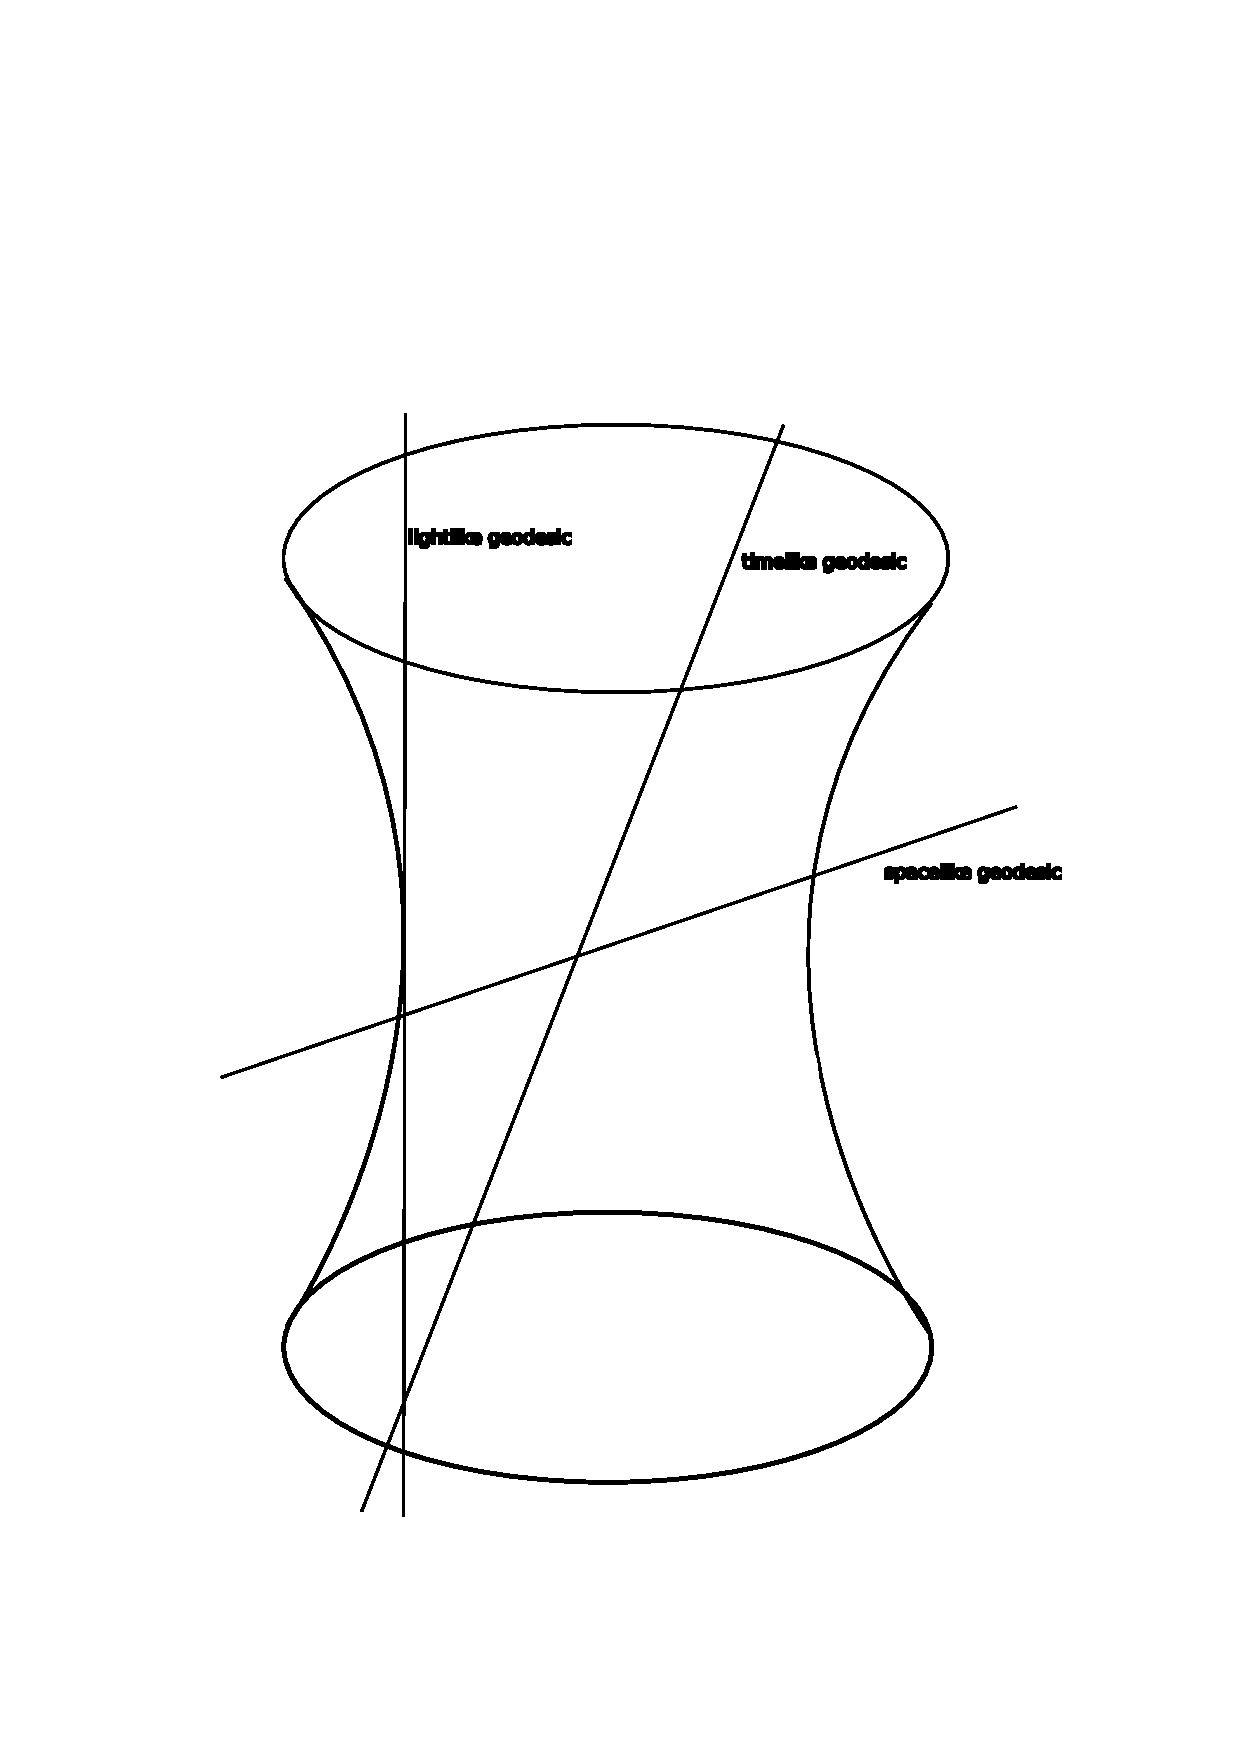
\includegraphics[width=0.5\textwidth]{projectivechart.pdf}
    \caption{Geodesics in $\A^{2,1}$}
    \label{projchart}
\end{figure}

%\begin{observation} Any timelike line is the projectivisation of a negative definite plane. As Isom$(\A^{n,1})\simeq \text{PO}(n,2)$ acts transitively on the space of timelike lines, and since the stabilizer of a timelike line is the group $\text{P}(O(n)\times O(2))$ which is the maximal compact subgroup of $\text{PO}(n,2)$, the space of timelike geodesics of $\A^{n,1}$ is naturally identified with the Riemannian symmetric space of PO$(n,2)$. \textcolor{red}{è una curiosità, non viene favvero utilizzato nel seguito, si potrebbe togliere.}
%\end{observation}

\subsection{Totally geodesic subspaces} Totally geodesic subspaces of $\A^{n,1}$ of dimension $k$ are obtained as the intersection of $\A^{n,1}$ with the projectivisation $\text{P}(W)$ of a linear subspace $W$ of $\R^{n,2}$ of dimension $k+1.$ The negative index of $W$ can be $1, 2,$ for otherwise the intersection $\A^{n,1}\cap \text{P}(W)$ would be empty. We have several cases: 
\begin{itemize}
    \item If $W$ has signature ($k-1$, 2), then $\text{P}(W)\cap \A^{n,1}$ is isometric to $\A^{k-1,1}$. 
    \item If $W$ has signature $(k-2, 1)$, then it is a copy of Minkowski space $\R^{k-2,1}$, hence $\text{P}(W)\cap \A^{n,1}$ is a copy of the Klein model of hyperbolic space. 
    \item If $W$ is degenerate, then $\text{P}(W)\cap \A^{n,1},$ is a lightlike subspace foliated by lightlike geodesics tangent to the same point of $\partial\A^{n,1}$. 
\end{itemize}  
A particular case of the last point is when $W$ is degenerate and $\text{dim}(W)=n+1.$ Then $\text{P}(W)\cap \A^{n,1}$ is a projective hyperplane tangent to $\partial\A^{n,1}$ at a point $[x]$ and $\text{P}(W)\cap \partial\A^{n,1}$ is the lightlike cone of $\partial\A^{n,1}$ through $[x]$.\\

\textit{In the universal cover.} In the universal cover $\AS^{n,1},$ geodesics are just the lifts of geodesics in $\A^{n,1}$ or $\H^{n,1}$. Hence, every spacelike or lightlike geodesic in $\A^{n,1}$ and $\H^{n,1}$, which is topologically a line, has a countable number of lifts to $\AS^{n,1}$. Timelike geodesics in $\A^{n,1}$ and $\H^{n,1}$ are topologically circles and are in bijections with timelike geodesics in $\AS^{n,1},$ as the covering map restricted to a timelike geodesic induces a covering map onto the circle. Using the Poincaré model we can give an explicit description of lightlike geodesics. In fact, in Lorentzian geometry not only the nature of a vector is conformally invariant but also unparametrized lightlike geodesics are a conformal property (\cite{Gallot}, Proposition 2.131): 
 \begin{theorem}\label{ConformalMetric} If two Lorentzian metrics $g,g^{\prime} $ on a manifold $M$ are conformal, then they have the same unparametrized lightlike geodesics.
 \end{theorem}

 Because of Theorem \ref{ConformalMetric} we can replace the Poincaré metric by the conformally equivalent -and often more easy to manage in calculation- metric given by:
 \begin{equation}\label{emispherical}
     \frac{4}{(1+r^2)^2}(dx_1^2+\dots+dx_n^2)-dt^2
 \end{equation} 
 Now we observe that the first term in Equation \ref{emispherical} is exactly the form of the spherical metric on a hemisphere, pulled-back to the unit disk by the stereographic projection. We will call such a metric hemispherical and will denote it by $g_{\mathbb{S}^n}$. Notice that the boundary of $\D^n$ is an equator for the hemispherical metric, and in fact it is the only equator completely contained in $(\D^n\cup\partial\D^n,g_{\mathbb{S}^n})$, a justification to the fact that we will refer to it as \textit{the} equator.\\
 As a consequence, unparametrized lightlike geodesics of $\AS^{n,1}$, going through a point $(p_0,t_0)$ are characterized by the condition that they are mapped to spherical geodesic under the vertical projection $(p,t)\to p$ and moreover: 
 \[
     t-t_0=d_{\mathbb{S}^n}(p,p_0)
 \] on the geodesic. In particular, these lightlike geodesics meet the boundary of $\AS^{n,1}$ at the point that satisfies the above conditions such that $p$ is on the equator of the hemisphere: as an example, if $p_0$ is the center of the hemisphere, then the points at infinity of the lightcone over $(p_0,t_0)$ are the horizontal slice $t=t_{0}+\pi/2.$ This sphere is also the boundary of a hyperplane dual to $(p_0,t_0)$, in a sense that we will explain in the following section. \\
 By an analogous reasoning we can give an explicit description of a lightlike hyperplane in the Poincaré model: the lightlike plane having $(p_0,t_0)$ as a past endpoint, (where now $p_0$ is on the equator) is precisely $\{(p,t)\;|\;t-t_0=d_{\mathbb{S}^n}(p,p_0)\}$ and its future endpoint is $(-p_0,t+\pi.)$ 

% \textcolor{red}{anche qua ci sarebbero le figure da inserire, imho queste sono effettivamente utili}

\section{Polarity in AdS}\label{polarsec}
The quadratic form $q_{n,2}$ induces a polarity on the projective space $\R\text{P}^{n+1}$, explicitly the correspondence associates to a projective subspace $\text{P}(W)$ the subspace $\text{P}(W^\perp)$. In particular, we have an induced duality between spacelike totally geodesic subspaces of $\A^{n,1}$ where the dual of a spacelike $k-$dimensional subspace is an $n-k+1$ subspace. \\
For instance, if we consider the dual of a point $[x]\in\A^{n,1}$ it will be an $n-$dimensional spacelike hyperplane $P_{[x]}=\text{P}(x^\perp).$ Projectively, $P_{[x]}$ is characterized as the hyperplane spanned by the intersection of $\partial\A^{n-1,1}$ with the lightcone from $[x]$. More geometrically, it can be checked that $P_{[x]}$ is the set of antipodal points to $[x]$ along timelike geodesics through $[x].$ Also, every timelike geodesic through $[x]$ meets $P_{[x]}$ orthogonally at time $\pi/2.$ Conversely, given a totally geodesic spacelike hyperplane $H$, all the timelike geodesics that meet $H$ orthogonally intersect in a single point, which is the dual point of $H$. 

 \subsection*{In the quadric model} We would like to \textit{lift} the idea of duality to coverings of $\A^{n,1}.$ Observe that in $\H^{n,1}$ there are two dual planes associated to any point $x$, namely the sets: 
 \[
     P_x^\pm=\{\exp_x(\pm(\pi/2)v)\;|\;q_{n,2}(v)=-1,\; v\;\text{future-directed}\}.
 \] 

 Now the points $P_x^+$ and $P_x^-$ are antipodal and $P_{-x}^\pm=P_x^\mp$. The planes $P_x^\pm$ disconnect $\H^{n,1}$ in two regions $U_x$ and $U_{-x},$ where $U_x$ is the connected component containing $x$. They can be characterized as: 
 \[
     U_x=\{y\in\H^{n,1}\;|\;\langle x,y\rangle_{n,1}<0\}.
 \]

 Spacelike and lightlike geodesics through $x$ do not exit $U_x$, while all the timelike geodesics through $x$ meet orthogonally $P_x^\pm$ and they all pass through the point $-x$. More precisely a point $y\neq x$ is connected to $x$: 
 \begin{itemize}
     \item by a spacelike geodesic if and only if $\langle x,y\rangle_{n,1}<-1,$
     \item by a lightlike geodesic if and only if $\langle x,y\rangle_{n,1}=-1,$
     \item by a timelike geodesic if and only if $|\langle x,y\rangle_{n,1}|<1.$ 
 \end{itemize}

 An immediate consequence is that if $y$ is connected to $x$ by a spacelike geodesic, there is no geodesic joining $y$ to $-x$. Hence the exponential map of $\H^{n,1}$ is not surjective. But as any point $y\in\H^{n,1}$ can be connected through a geodesic either to $x$ or $-x$ it follows that the exponential over $\A^{n,1}$ is surjective.
% \subsection{In the universal cover}
% Recall that $\AS^{n,1}\simeq \H^n\times\R$ with the group of deck transformations being isomorphic to $\Z$, where a generator acts by translation of $2\pi$ in the $\R$ factor. It follows that the preimage of a spacelike plane $P\subset\A^{n,1}$ is the disjoint union of spacelike planes $(P^k)_{k\in\Z},$ enumerated so that the generator $\eta$ of $\Z$ acts by sending $P^k$ to $P^{k+1}.$ \\
% Each connected component of $\AS^{2,1}\setminus\bigcup_{k\in\Z} P^k$ is a fundamental domain for the action of deck transformations of the covering $\AS^{n,1}\to\A^{n,1}.$ Given a point $x$, let us apply the previous construction to the plane $P_x=P_{\pi^{\prime}(x)}$ which is the dual of the image $\pi^{\prime}(x)$ in $\A^{n,1}$, and let $V_x$ be the connected component which contains $x$. We will refer to $V_x$ as the \textit{Dirichlet domain} in $\AS^{2,1}$ centered at $x$, since the construction of $V_x$ is the analogue of a Dirichlet domain to our context. Then the restricted covering map: $\restr{\pi^{\prime}}{V_x}:V_x\to\A^{2,1}\setminus P_x$ is an isometry, therefore lightlike and spacelike geodesic through $x$ are entirely contained in $V_x$.\\ 

% \textcolor{red}{Anche qua le immagini sono utili }